\section{Results}

OVERVIEW
For as long as the animal is not at the goal position:
\begin{tcolorbox}
\begin{enumerate}
    \item The animal makes a decision (and this decision is recorded)
    \item Non-non animal robot steps back from Non-animal robot
    \item Non-non animal robot path-finds to the pathfinding target
    \item Non-animal robot steps back from Non-animal robot
    \item Non-animal robot path-finds to the pathfinding target
    \item When both the robots are in the correct outer ring positions, they both move to the inner ring.
\end{enumerate}
\end{tcolorbox}



\subsection{Control flow diagram of the algorithm}
\begin{figure}[H]
    \centering
    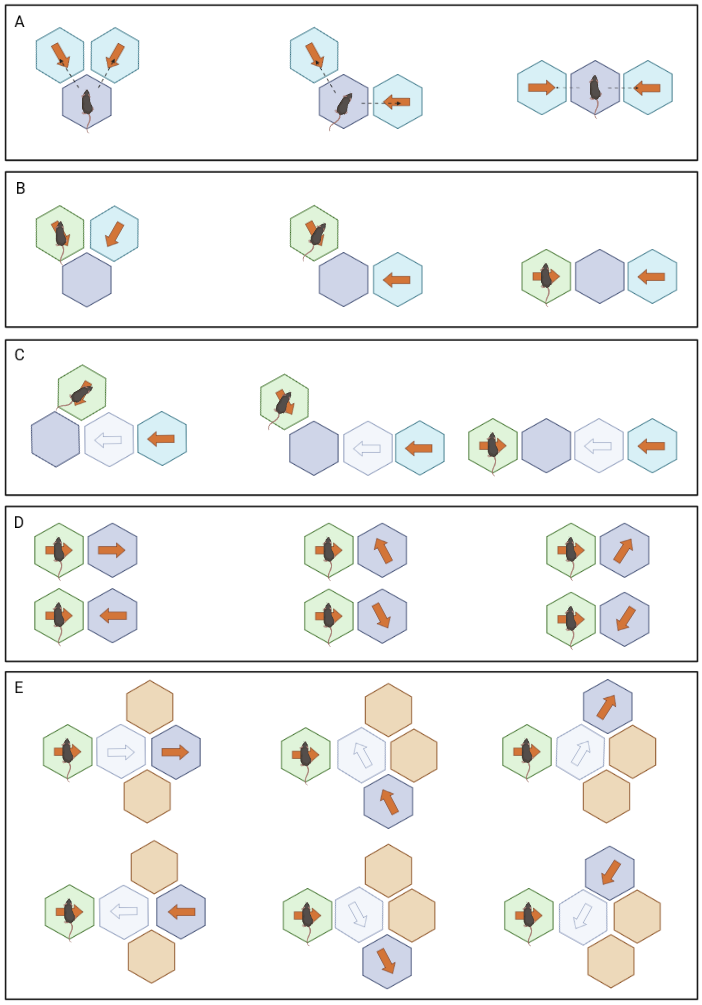
\includegraphics[scale = 1.4]{images/control_flow_diagram.png}
    \caption{Control Flow Diagram of algorithm that has been implemented. \textbf{A} shows the possible states of the platforms, the mouse will be presented to decide which one to move to. Before this happens there is no difference between the \textit{NAR} and \textit{NNAR} so they are both coloured the light blue. Once the animal has made a decision, the \textit{NAR}(in dark blue), the \textbf{AR} (in green) and \textit{NNAR} robots (in light blue) are labeled appropriately. \textbf{C} shows that from all possible arrangements of the platforms, the \textit{NNAR} (labelled light blue), must move backwards so that it does not intersect with the other robots when pathfinding away. \textbf{D} shows is the two consecutive platforms, with their directions labeled (in all possibilities for the dark blue robot. From \textbf{E}, it can be seen that for all the possible cases of the blue's orientation compared with the green, the \textit{NAR} must always move to the (orange) \textit{outer ring}.}
    \label{fig:control_flow_diagram}
\end{figure}

\begin{algorithm}
\caption{Instantiating the environment}
\begin{algorithmic}

\STATE hm = HexagonMaze(rows, columns, *name) \Comment{Instantiate the Maze Class}

\STATE
\STATE robot1 = PlatformRobot(x-position, y-position, z-position, direction, IP address, *name) 
\STATE robot2 = PlatformRobot(x-position, y-position, z-position, direction, IP address, *name) 
\STATE robot3 = PlatformRobot(x-position, y-position, z-position, direction, IP address, *name) 

\STATE
\STATE mouse = Animal(Maze, *name)

\STATE
\STATE Place the animal on a robot

\STATE
\STATE Run the main loop of the program

\end{algorithmic}
\end{algorithm}

\begin{algorithm}
\caption{The main loop for the overall program}
Animal Robot makes decision for which platform to choose \\

\WHILE{Animal is not at Goal}
\STATE The Animal robot changes state \\ 

\STATE NNAR steps backwards \\ 
\STATE NNAR get its new outer ring target position \\
\STATE NNAR finds the shortest path between its current position and the outer ring position \\


\STATE NAR steps into the outer ring \\
\STATE NAR gets its new outer ring target position \\
\STATE NAR finds the shortest part between its curre




\end{algorithm}

